\documentclass[12pt]{report}
\usepackage[top=2cm, bottom=2cm, left=3cm, right=1.5cm]{geometry}

\usepackage{fontspec}
\usepackage{polyglossia}
\setdefaultlanguage{russian}
\newcommand{\docfont}{Times New Roman}
\setmainfont[Ligatures=TeX]{\docfont}
\newfontfamily\cyrillicfont[Ligatures=TeX]{\docfont}
\newfontfamily\cyrillicfontsf[Ligatures=TeX]{\docfont}
\newfontfamily\cyrillicfonttt[Ligatures=TeX]{\docfont}

\usepackage[plain]{algorithm}
\usepackage[noend]{algpseudocode}
\renewcommand{\algorithmiccomment}[1]{{\quad\footnotesize // #1}}
\renewcommand{\algorithmicrequire}{\textbf{Input:}}
\renewcommand{\algorithmicensure}{\textbf{Output:}}

\usepackage{amsmath,amsfonts,amsthm,amssymb} % nice math symbols
\newtheorem{definition}{Определение}

\usepackage{hyperref}
\hypersetup{%
	pdfencoding=auto,
	pdfauthor={Александр Панов},
	pdftitle={Отчет РФФИ мол_а_дк}
}

\usepackage[
	autolang=hyphen,
	language=auto,
	autolang=other,
	backend=biber,
	style=gost-numeric
]{biblatex}
\addbibresource{rfbr_moladk_2016.bib}

\DeclareSourcemap{
	\maps[datatype=bibtex, overwrite]{
		\map{
			\step[fieldset=langid, fieldvalue=english]
			\step[fieldset=doi, null]
			\step[fieldset=issn, null]
			\step[fieldset=isbn, null]
			\step[fieldset=url, null]
			\step[fieldsource=language, fieldset=langid, origfieldval]
		}
	}
}

\usepackage{graphicx}
\graphicspath{{../../images/}}

\title{Развернутый научный отчет}
\author{А.\,И.~Панов}

\begin{document}
	\maketitle
	\setcounter{chapter}{3}
	\section{Номер проекта}
	16-37-60055 мол\_а\_дк
	
	\section{Название Проекта}
	Исследование механизмов и построение моделей обучения, основанных на знаковых представлениях, в задаче планирования коллективного поведения
	
	\section{Коды классификатора, соответствующие содержанию фактически проделанной работы}
	\begin{itemize}
		\item 07-991 Интеллектуальные динамические системы и технологии управления
		\item 07-966 Методы и системы приобретения, представления, обработки и интеграции знаний
	\end{itemize}

	\section{Объявленные ранее цели Проекта}
	Первый год работ по проекту (2016 г.): 
	\begin{enumerate}
		\item Исследование структуры внутренней процедурной компоненты элементов семиотического представления знаний (знаков) интеллектуального агента, действующего в условиях коллективного решения поставленной задачи. 
		\item Исследование взаимосвязи процессов целеполагания в условиях коллективного взаимодействия и процесса функционирования внутренней процедурной компоненты знака. 
		\item Подготовка публикаций в ведущих периодических изданиях, включенных в одну из систем цитирования (библиографических баз) Web of Science, Scopus, РИНЦ.
	\end{enumerate}
	
	\section{Полученные в 2016 году результаты с описанием методов и подходов, использованных в ходе выполнения проекта}
	
	На первом этапе проекта основной целью работ являлось исследование внутренней процедурной компоненты знаков интеллектуального агента, действующего в условиях коллективного решения задачи. Рассматривалась модель основного когнитивного процесса, задействованного при составлении решения задачи, в том числе в коллективе, --- процесс планирования с включением этапа целеполагания. Была разработана модель процедурной компоненты знака и исследована его роль в процессе планирования, алгоритм которого был развит на основе предыдущих работ автора.
	
	\subsection{Моделирование процесса планирования поведения}
	
	Вопрос разработки методов планирования поведения сложного технического или виртуального объекта имеет большую историю и в основном связывается с успехами отдельной области искусственного интеллекта - автоматического планирования. Здесь достигнуты существенные успехи - предложен ряд символьных методов планирования как в классической постановке задачи, когда действия детерминированы (такие алгоритмы планирования, как FF \cite{Hoffmann2001}, FD \cite{Helmert2006}, LAMA \cite{Richter2010}), так и в недетерминированной постановке с учетом ненулевых вероятностей невыполнения действий и вероятностной реакции среды (алгоритмы на основе марковских процессов и динамического программирования \cite{Barto1995,Bonet2009}). Однако создание эффективных и быстрых алгоритмов планирования действий основывается на заранее заданных эвристических принципах поиска на графе и на предположении, что набор действий заранее известен, что делает невозможным автоматическую адаптацию системы планирования к новой задаче с новым списком действий. Это означает, что переноса опыта планирования с выделением абстрактных действий, которые могут иметь различную реализацию в разных ситуациях, в классических подходах не происходит. Существенные трудности возникают, когда существующие алгоритмы адаптируются для многоагентного случая, где предполагается, что агенты обладают как различными наборами действий, так и обладают различными знаниями о внешней среде \cite{Brafman2015}. В случае коалиционного взаимодействия также необходимо обязательное включение элементов обучения для пополнения базы данных одного агента по поступающей от других участников коалиции информации.
	
	В последнее время исследователи в области управления и планирования уделяют повышенное внимание психологически и биологически правдоподобным моделям и архитектурам управления агентами \cite{Kelley2006,Sun2012a}. Использование различных типов памяти (эпизодической, процедурной и др.) в когнитивных архитектурах нацеленно именно на задачу повторить биологические и психологические пути обмена и организации информации для решения таких задач как управление и планирование поведения. Это связано в первую очередь с тем, что повышающийся уровень сложности тех задач, в которых действуют робототехнические системы (агенты) требует от них большего уровня автономности, универсальности и гибкости, которую не могут обеспечить существующие методы и алгоритмы. Исследователи в области искусственного интеллекта снова обращаются к естественным примерам решения таких задач - к исследованию поведения человека и животных \cite{Redko2016,Panov2016d}. Психологически правдоподобные модели когнитивных функций, в том числе планирования, нацелены не только на то, чтобы повторить поведение человека в сложных, в том числе коалиционных, условиях, но и по возможности более полно удовлетворить существующим психологическим представлениям о функционировании психики человека. С одной стороны это может привести к повышению ресурсоемкости предлагаемых алгоритмов, но, с другой стороны, позволит реализовать новые возможности, которые раньше оставались вне круга решаемых проблем специалистами по планированию, например, возможности к целеполаганию, распределению ролей в коллективе. Идеи когнитивной психологии и раньше использовались в классическом планировании, но, в основном, в бихевиориостском ключе. Так идея в разделении множества действий на автоматические, быстро совершаемые, специфические и произвольные, обобщенные, подсказанное психологической теорией \cite{Kahneman2011}, нашла свое воплощение в иерархическом планировании, а идея сохранения опыта планирования - в прецедентном \cite{Hammond1990,DeLaRosa2013,Borrajo2015}.
	
	В когнитивной психологии имеется ряд направлении, изучающих феномен планирования, среди которых необходимо выделить три основных \cite{Chuvgunova2015}: планирование как часть когнитивной схемы \cite{Neisser1976}, планирование как метапроцесс \cite{Flavell1979,Sternberg2000} и планирование как часть деятельности \cite{Leontiev1977}. В первом направлении для описания поведения человека используются когнитивные схемы. Например, перцептивная схема – это план сбора информации об объектах и событиях, получения новой информации, обеспечивающий ее непротиворечивую интерпретацию. Схема одновременно включает в себя и сам план, и исполнение плана, это структура действия, равно как и структура для действия. Во втором направлении предусматривается наличие метакогнитивных процессов, позволяющих человеку управлять своими когнитивными процессами и знаниями. С точки зрения Стернберга, можно говорить о глобальном (стратегическом) и локальном (тактическом) планировании. Глобальное планирование требует больших затрат времени, но это компенсируется уменьшением времени на локальное, тактическое планирование. Наконец, в третьем подходе, являющимся одним из наиболее общих, рассматривается иерархическая теория деятельности, которая используется в данном проекте и описывается в следующем разделе.
	
	Стоит отметить также, что психологически и биологически правдоподобные модели управления и планирования позволяют по-другому взглянуть на проблему символизации (symbol grounding problem) \cite{Harnad1990,Barsalou1999,Chella2003,Besold2015}. Нейрофизиологические модели функционирования сенсорных отделов коры головного мозга в купе с психологической теорией категоризации и восприятия служат основой для построения новых непротиворечивых моделей привязки символов к сенсорным данным. Успехи в данном направлении позволили реализовать некоторые модели в робототехнических системах \cite{Heintz2010}. 
	
	Далее будет представлен новый психологически и биологически правдоподобный метод планирования поведения, основанный на знаковой теории деятельности и моделях строения кортикально-таломических отделов коры головного мозга. Помимо своей ценности с точки зрения моделирования когнитивных функций человека знаковый подход может быть использован при решении ряда коллективных робототехнических задач (например, для задача интеллектуального перемещения \cite{Panov2015g,Panov2016d}), не решаемой классическими и другими психолого ориентированным методами (такими как BDI \cite{Sardina2006}).
		
	\subsection{Знаковая картина мира}\label{sec:swm}
	
	В качестве способа представления знаний в настоящем проекте используется модель знаковой картины мира \cite{Osipov2014c,Osipov2015b, Osipov2016}, которая не только хранит знания об объектах, процессах и отношениях внешней среды, но также представляет внутренние параметры интеллектуального агента, определяющие его мотивационную составляющую и опыт действования. Картина мира также включает в себя процедуры оперирования со знаниями: их приобретение и использование в различных процессах, таких как восприятие, рассуждения, целеполагание, планирование поведения\cite{Osipov2015d}. Модель картины мира строится на основе психологических представлений о функционировании психики человека, в частности на представлениях культурно-исторического подхода \cite{Vygotsky1999}, теории деятельности \cite{Leontiev1977,Chudova2012b} и теории дуальных систем \cite{Evans2013,Stanovich2009}. В соответствии с психологическими воззрениями элементом картины мира является четырехкомпонентная структура - знак, которая представляет для субъекта (в нашем случае интеллектуального агента) все сущности внешней среды и внутреннего пространства: объекты, их свойства, процессы, отношения между объектами и процессами. Следует отметить, что знак является продуктом взаимодействия нескольких субъектов деятельности, образующих некоторую группу (культурную среду), т.е. понятие знака изначально предполагает работу картины мира индивида в кооперации с картинами мира других индивидов.
	
	Образная компонента знака хранит характерные признаки представляемой сущности и одновременно является функцией построения представления этой сущности на основе потока данных, поступающих как с наружных, так и внутренних сенсоров, и в котором выделяются ключевые признаки. Образная компонента индивидуальна для каждого носителя картины мира и образуется в результате процесса наблюдения и обобщения \cite{Panov2014d,Panov2015c,Skrynnik2016}. 
	
	Компонента значения знака представляет обобщенные, концептуальные знания субъекта о сущностях внешней среды, а также внутреннего пространства как себя, так и других участников группы. Эти знания являются согласованными, т.е. одинаковы у всех представителей группы. Коммуникативные процессы, которые протекают в группе субъектов (интеллектуальных агентов), в своей основе используют сообщения, которые строятся по общим для всех значениям знаков, задающих, таким образом, синтаксис протокола коммуникации.
	
	Компонента личностного смысла знака содержит индивидуальный личный опыт взаимодействия субъекта с внешней средой с учетом отношения к этому опыту - послужил ли он достижению некоторой цели (удовлетворению некоторой потребности), или же наоборот, оказался неудачным. Личностный смысл знака является динамической его характеристикой, которая постоянно формируется и обновляется в результате протекания тех или иных когнитивных процессов (планирования, целеполагания). Именно компонента личностного смысла определяется внутренними характеристиками субъекта и его потребностно-мотивационной сферой.
	
	Наконец, четвертая компонента знак - имя - служит для его идентификации как в коммуникативных процессах, так и в произвольных процессах планирования и рассуждений. Имя знака, как и его значение, является утвержденной, слабо меняющейся в группе субъектов компонентой знака.
	
	Знаки представляет в картине мира субъекта как статические объекты и свойства внешней среды, так и динамические ее составляющие: процессы, ситуации - а также внутренние характеристики агента: действия, объекты и свойства <<внутренней среды>>. Пусть у нас есть объект внешней среды - \textit{лимон}. В картине мира некоторого субъекта он может представляться знаком с именем <<лимон>>, образ которого включает такие признаки как \textit{желтый цвет}, \textit{овальную форму} и \textit{кислый вкус}. Эти признаки также могут быть представлены в картине мира знаками, либо являться информацией, поступающей напрямую от сенсоров. Значением знака <<лимон>> будут являться те обобщенные действия и процессы, в которых по общему согласованному мнению некоторого коллектива, которому принадлежит субъект, участвует \textit{лимон}: лимон \textit{принято употреблять в пищу}, \textit{использовать как соус для рыбных блюд} или \textit{использовать для профилактики болезней}. Личностный смысл лимона для субъекта - это те конкретные персональные действия и процессы, в которых субъект имел опыт использования лимона, решая некоторую задачу: когда-то я \textit{кидал лимон в соседа по парте в школе} или \textit{сжевал целый лимон и не скривил лицо}. Все действия и процессы также могут быть представлены некоторыми знаками, либо не выводиться на знаковый произвольный уровень и являться некоторыми не обозначаемыми операциями.
	
	Кроме психологических оснований четырхекомпонентной структуры знака имеются нейрофизиологические свидетельства в пользу существования такой структуры хранения и активации элементов индивидуального опыта \cite{Edelman1987,Ivanitsky1996}. Кроме того, нейрофизиологические данные служат основной для построения моделей компонент знака и некоторых функций, таких как восприятие и распознавание \cite{George2009,Panov2014d}. Нейрофизиологические свидетельства в пользу высокой однородности строения различных отделов коры больших полушарий мозга, а также участия таламуса в формировании и запоминании временных последовательностей \cite{Buxhoeveden2002,Constantinople2013}, приводят к используемой в данном проекте  математической структуре каузальной матрицы \cite{Panov2015c} для описания строения компонент знака.
	
	Знаковый подход к представлению знаний и описание процессов, протекающих в знаковой картине мира позволяют решить ряд трудных задач в области ситуационного управления \cite{Osipov1999,Osipov2002c} и управления сложными техническими объектами \cite{Zubarev2013}. Использование знаковой картины мира для реализации функций стратегического уровня управления робототехническими системами \cite{Makarov2015a} демонстрирует применимость используемого подхода не только для представления знаний, но и для решения задач коалиционного планирования и распределения ролей.
	
	\subsubsection{Компоненты знака}\label{subsec:components}
	
	Рассмотрим структуру компонент знака на примере образной компоненты, которая участвует в распознавании (актуализации) знака, выделении представления об опосредуемом объекте или процессе на основе поступающей из внешней среды сенсорной информации и регистрируемой внутренними сенсорами моторной информации. До именования знак будем называть протознаком или признаком.
	
	Предположим, что во входном потоке данных выделена последовательность $(x_1,x_2,\dots,x_h)$ длины $h$ векторов действительных чисел от 0 до 1, которые будем называться \textit{событиями}. Каждое событие $x_t$ длины $q$ представляет собой запись выходов от $q$ сенсоров, а каждый элемент события означает уверенность в срабатывании данного сенсора. Например, событие $(0.1, 0.9, 0.9)$ поступает с трех сенсоров - датчиков красного, синего и зеленого света - и означает, что уверенность в срабатывании датчика красного света составляет 10\%, а синего и зеленого - по 90\%.
	
	Образная компонента знака должна по входной последовательности данных определить, присутствует ли (закодирован ли) опосредуемый объект или процесс в этой последовательности. Для этого мы будем кодировать характерные признаки объекта или процесса в специальной структуре - каузальной матрице $z=(e_1,e_2,\dots,e_h)$ размерности $q$ на $h$, где $q$ - размерность входных событий, а $h$ - длина последовательности входных событий. При этом каждый столбец $e_t$ каузальной матрицы является битовым вектором длины $q$ и кодирует те признаки (которым соответствуют 1), которые необходимо должны присутствовать во входном событии в момент времени $t$, чтобы опосредуемый объект или процесс мог быть распознан во входном потоке данных, т.е. задают множество одновременных характерных признаков. Например, образу знака $s$, представляющему объект <<квадрат>>, может соответствовать каузальная матрица 
	\[
	\renewcommand\arraystretch{0.5}
	z=\begin{bmatrix}
	1&1&1&1\\
	0&1&1&0\\
	1&0&0&1\\
	1&1&0&0\\
	0&0&1&1
	\end{bmatrix},
	\]
	где первая строчка является характеристическим вектором информации с датчика углов на изображении, вторая - с датчика положения визуального сенсора (верхнее положение), третья - нижнее положение сенсора, четвертая - левое положение сенсора, пятая - правое положение (см. рис.\ref{fig:square}).
	
	\begin{figure}
		\label{fig:square}
		\centering
		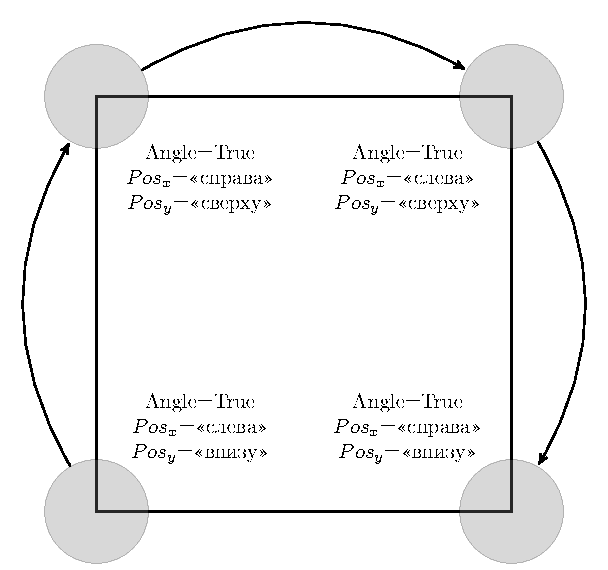
\includegraphics[width=0.5\textwidth]{examples/recognition/square}
		\caption{Визуальная интерпретация каузальной матрицы}		
	\end{figure}
	
	Образу каждого знака может соответствовать несколько каузальных матриц, которые задают различные проявления представляемого объекта или процесса. Весь кортеж каузальных матриц образа знака $s$ будем обозначать как $Z^p(s)$. 
	
	Случай, когда характерными признаками образа данного знака выступают данные с сенсоров, является частным. В более общей постановке, признаками для образа знака служат другие знаки, которые представляют эти характерные признаки. Таким образом, мы можем сопоставить образу знака $s$ множество $S_p(s)$ мощности $q$, каждому элементу которого соответствует номер строчки каузальной матрицы $z$ размера $q$ на $h$, т.е. каждому признаку $s_i\in S_p(s)$ соответствует характеристический битовый вектор, задающий на местах 1 те моменты времени, когда данный признак должен присутствовать во входных данных, чтобы успешно актуализировать знак (распознать образ знака) $s$. 
	
	Для уточнения определения множества $S_p(s)$ введем семейство бинарных отношений $\{\sqsubset_p,\sqsubset_p^1,\sqsubset_p^2,\dots\}$, определённых на декартовом произведении $S\times S$. Будем считать, что знак $s_i$ является \textit{элементом образа} знака $s$, $(s_i,s)\in\sqsubset_p$ или $s_i\sqsubset_p s$, в том случае, если $s_i\in S_p(s)$. Если известно, что знаку $s_i$ соответствует 1 в $t$-м столбце некоторой каузальной матрицы $z\in Z^p(s)$ знака $s$, то мы будем использовать вложенное отношение $\sqsubset_p^t\subset \sqsubset_p$.
	
	\subsubsection{Каузальная сеть} \label{subsec:causal_net}
	
	Введем специальную процедуру $\Lambda_p: 2^Z\rightarrow 2^{\mathbb N}\times 2^{\mathbb N}$, которая каждому кортежу каузальных матриц $Z^p(s)\subset Z$ образа знака $s$ ставит в соответствие два не пересекающихся подмножества индексов собственных столбцов $I^c\subset\mathbb N, \forall i\in I^c\ i\leq h$ (индексы столбцов условий) и $I^e\subset\mathbb N, \forall i\in I^e\ i\leq h$ (индексы столбцов эффектов): $\Lambda_p(Z^p(s))=(I^c,I^e), I^c\cap I^e=\varnothing$. Например, если для множества матриц $Z=\{((1, 0), (0, 1))\}$ процедура $\Lambda_p$ выдает два множества $\{1\}$ и $\{2\}$, то это означает, что появление признака, соответствующего первой строчке матрицы, вызывает появление признака, соответствующего второй строчке. Процедура $\Lambda_p$ по сути является функцией установления причинно-следственного отношения на множестве входных событий и может реализовываться различными способами, в т.ч. на основе алгоритмов Норриса, FCbO, AddIntent (\cite{Norris1978,Krajca2010,Merwe2004})
	
	В том случае, когда для матриц $Z^p(s)$ образа знака $s$ множество столбцов эффектов пусто $I^e=\varnothing$, т.е. когда по данному множеству каузальных матриц не возможно однозначно определить, какие события всегда предшествуют другим, мы будем считать, что причинно-следственная связь не установлена и знак опосредует некоторый объект или ситуацию. В противном случае будем считать, что знак опосредует некоторое действие или процесс, результат которого кодируется в столбцах эффектов, а условие - в столбцах условий. 
	
	\begin{figure}
		\centering
		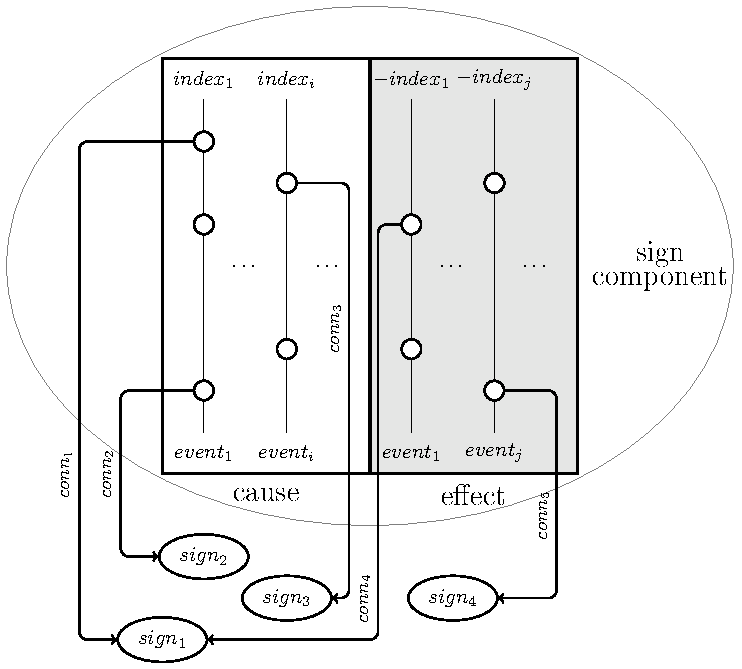
\includegraphics[width=0.6\textwidth]{causnet/caus_matr}
		\caption{Схема каузальной матрицы}	
		\label{fig:caus_matr}	
	\end{figure}
	
	Справедливы следующие утверждения относительно свойств процедуры $\Lambda_p$:
	\begin{itemize}
		\item $I^c\cap I^e=\varnothing$ --- столбец матрицы предсказания не может быть одновременно и условием и эффектом,
		\item $|I^c\cup I^e|=h$ --- столбец матрицы предсказания является либо условием либо эффектом,
		\item $I^c\not = \varnothing$ --- среди столбцов матрицы предсказания должен быть хотя бы один столбец условий, в то время как эффектов может и не быть (в случае объектных признаков),
		\item $\forall i\in I^e, j\in I^c\ i>j$ --- все условия предшествуют эффектам по времени.
	\end{itemize}
	
	Схема каузальной матрицы, с учетом выше сказанного, приведена на рис. \ref{fig:caus_matr}.
	
	Теперь введем понятие каузальной сети, которая будет определять гетерархию на множестве образов. Каузальная сеть $W_p=\langle V_p, E_p \rangle$ - является помеченным ориентированным графом, в котором
	\begin{itemize}
		\item каждому узлу $v\in V_p$ ставится в соответствие кортеж казуальных матриц $Z^p(s)$ образа некоторого знака $s$, что будем обозначать как $v\rightarrow Z^p(s)$;
		\item ребро $e=(v_1, v_2)$ принадлежит множеству ребер графа $E$, если $v_1\rightarrow Z^p(s_1), v_2\rightarrow Z^p(s_2)$ и $s_1\in S_p(s_2)$, т.е. если знак $s_1$ является элементом образа знаком $s_2$;
		\item каждому ребру графа $e=(v_1, v_2), v_1\rightarrow Z^p(s_1), v_2\rightarrow Z^p(s_2)$ ставится в соответствие метка $\epsilon=(\epsilon_1,\epsilon_2,\epsilon_3)$ - кортеж трех натуральных чисел:
		\begin{itemize}
			\item $\epsilon_1$ - индекс исходной матрицы в кортеже $Z^p(s_1)$, может принимать специальное значение 0, если исходными могут служить любые матрицы из кортежа;
			\item $\epsilon_2$ - индекс целевой матрицы в кортеже $Z^p(s_2)$, строка которой ставится в соответствие признаку $s_1$;
			\item $\epsilon_2$ - индекс столбца в целевой матрице, в которой в соответствующей признаку $s_1$ строке стоит 1, может принимать положительные значения (столбцы условий) и отрицательные (столбцы эффектов).
		\end{itemize}		
	\end{itemize}
	
	Каузальная сеть представляет собой некоторое множество пересекающихся иерархий знаков. Каждый знак представлен множеством каузальных матриц, задающих образ этого знака, а иерархия представляет иерархические связи между образами. Такую связь можно читать как <<знак $x$ участвует в формировании образа знака $y$>>. При этом мы специфицируем для какой именно матрицы знака $y$ и какого именно столбца этой матрицы нужен знак $x$ (метки $\epsilon_2$ и $\epsilon_3$ соответственно). В некоторых случаях мы также можем указать и участвующую в процессе формирования образа матрицу знака $x$ (метка $\epsilon_1$). Пример такой сети изображен на рис. \ref{fig:caus_net}.
	
	Аналогичным образом определяются каузальные сети для остальных компонент знака - для значения и личностного смысла. Для каждого знака $s$ задаются множества $S_m(s)$ и $S_a(s)$, т.е. определяются семейства отношений $\{\sqsubset_m,\sqsubset_m^1,\sqsubset_m^2,\dots\}$ и $\{\sqsubset_a,\sqsubset_a^1,\sqsubset_a^2,\dots\}$. Множество $S_m(s)$ интерпретируется как ролевой состав знака $s$, например, элементы подкласса или роль действия. Множество $S_a(s)$ интерпретируется как мгновенный компонентный состав некоторой ситуации, наблюдаемой и переживаемой субъектом, носителем картины мира, в настоящее время. Аналогично определяются множества $Z^m(s)$, $Z^a(s)$, процедуры $\Lambda_m$ и $\Lambda_a$.
	
	\begin{figure}
		\centering
		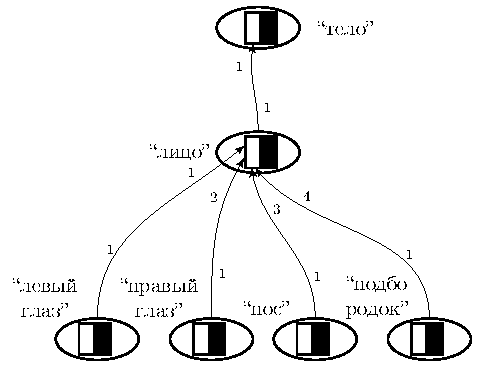
\includegraphics[width=0.5\textwidth]{examples/causnet/caus_net}
		\caption{Схема каузальной сети. Здесь каузальные матрицы изображены в виде квадратов, столбцы условий - левая белая часть квадрата, столбцы эффектов - черная правая часть квадратов. Метка $\epsilon_1$ отображается в начале каждой стрелки, метка $\epsilon_2$ определяется как номер квадрата, к которому идет стрелка, а метка $\epsilon_3$ отображается в конце каждой стрелки.}
		\label{fig:caus_net}		
	\end{figure}
	
	\subsection{Семиотическая сеть} \label{sec:semiotics}
	
	Знаком $s$ будем называть четверку $\langle n, p, m, a\rangle$, где $n$ - имя знака, $p$ - образ знака, кортеж каузальных матриц $\langle z_1^p(s), z_2^p(s), \dots\rangle$, соответствующий узлу $w_p(s)$ каузальной сети на образах;  $m$ - значение знака, кортеж каузальных матриц $\langle z_1^m(s), z_2^m(s), \dots\rangle$, соответствующий узлу $w_m(s)$ каузальной сети на значениях,  $a$ - личностный смысл знака, кортеж каузальных матриц $\langle z_1^a(s), z_2^a(s), \dots\rangle$, соответствующий узлу $w_a(s)$ каузальной сети на смыслах.
	
	Будем называть \textit{семиотической сетью} пятерку $\Omega=\langle W_p, W_m, W_a, R_n, \Theta \rangle$, где
	\begin{itemize}
		\item $W_p, W_m, W_a$ - соответственно каузальные сети на множестве образов, значений и личностных смыслах,
		\item $R_n$ - семейство отношений на множестве знаков, сгенерированных на основе трех каузальных сетей, т.е. $R_n=\{R_p, R_m, R_a\}$,
		\item $\Theta$ - семейство операций на множестве знаков, которые  генерируются на основе структуры фрагментов трех типов каузальных сетей, к которым принадлежат соответствующие компоненты знаков (подробнее см. \cite{Osipov2014c}).
	\end{itemize} 
	
	Еще раз отметим, что знак представляет не только объекты внешнего мира, но также процессы, протекающие в нем, выполнимые действия, а также ситуации, наблюдаемые во внешней среде.
	
	Три типа каузальных сетей, составляющих семиотические сеть, не независимы друг от друга. Между узлами каждой сети установлено взаимно-однозначное соответствие: для каждого узла $w_x$ сети $W_x$ найдутся единственные узлы $w_y$ и $w_z$ в сетях $W_y, W_z$ ($x,y,z\in\{p,m,a\}$), такие, что все три узла соответствуют одному и тому же знаку $s=\langle w_p, w_m, w_a\rangle$. Имя знака служит меткой узлов в каждой сети: в каузальной сети может быть только один узел с данной меткой, а узлы всех сетей с одинаковыми метками образуют компоненты знака. Для связи каузальных матриц различных типов узлов в рамках одного знака служат специальные функции связывания: $\Psi_p^m, \Psi_m^a,\Psi_a^p$ и обратные им $\Psi_m^p,\Psi_a^m,\Psi_p^a$ \cite{Osipov2014c}. Каждая функция связывания ставит каузальной матрице одного типа каузальную матрицу другого типа либо генерирует эту матрицу в том случае, если она отсутствует в соответствующем узле сети.
	
	Введем понятия активности в семиотической сети и процесса его распространения. Введем некоторую метку активности для каузальных матриц сети $W_x$ ($x\in\{p,m,a\}$) и будем называть активным множество $Z_x^*$ матриц, обладающих этой меткой. Процесс распространения активности представляет собой изменение состава  множества $Z_x^*$ с течением времени (каждый дискретный момент) и описывается для каждого типа каузальной сети своей функцией: $\varphi_a, \varphi_m,\varphi_p$. Процесс распространения активности является итерационным, т.е. на каждом шаге новый состав множества активных матриц порождается на основе предыдущего состава и зависит от матриц, туда входящих. В простейшем случае мы будем рассматривать такой процесс, в котором каждая матрица не влияет на ход распространения активности от другой матрицы и поэтому будем считать, что функции $\varphi_x$ принимают на вход одну активную  матрицу и выдают новое подмножество активных матриц. 
	
	В связи с тем, что ребра каузальных сетей имеют направлением, будем различать распространение активности вверх по сети, когда используются исходящие от узла ребра (функции $\varphi_x^\uparrow$), и распространение активности вниз по сети, когда используются входящие в узел ребра (функции $\varphi_x^\downarrow$). В дальнейшем, при описании алгоритма планирования, нам понадобятся только функции на сети значения и личностных смыслов. Каждую функцию $\varphi_x^\uparrow,\varphi_x^\downarrow$ будем параметризовать глубиной распространения активности $d_x$, которая указывает на какую глубину просматриваются ребра в данном направлении (вверх или вниз).
	
	В дальнейшем при описании алгоритма планирования будет использоваться понятие фрагмента казуальной сети. Под фрагментом $F$ мы будем подразумевать некоторое множество узлов $V$ сети $W_x=\langle V_x,E_x\rangle$ вместе со всеми ребрами $E$ их связывающими: $F=\langle V,E\rangle: V\subseteq V_x$ и $\forall e=(v_1,v_2)\in E v_1\in V, v_2\in V$.
	
	\subsection{Планирование в знаковой картине мира с этапом целеполагания}\label{sec:plan}
	
	Процесс планирования в знаковой картине мира реализуется с помощью MAP-алгоритма и идет в обратном направлении: от конечной ситуации к начальной. Кратко опишем основные этапы его работы. На вход алгоритма поступает описание задачи 
	\[T = \langle N_T,S,Sit_{start}, Sit_{goal}\rangle,\]
	где $N_T$ - идентификатор задачи, $S$ - множество знаков семиотической сети, $Sit_{start}=\langle \varnothing, \varnothing, a_{start} \rangle$ - начальная ситуация со смыслом $a_{start}=\{z_{start}^a\}$, $Sit_{goal}=\langle \varnothing, \varnothing, a_{goal} \rangle$ - целевая ситуация со смыслом $a_{goal}=\{z_{goal}^a\}$. В общем случае задача $T$ является результатом процедуры <<означивания>> - формирования картины мира по исходным описаниям домена планирования $D$, задающему списки возможных действий и типов объектов, и задачи планирования $P$, включающей в себя определение стартовых условий и конечной цели (шаг \ref{alst:ground}).
	
	Результатом MAP-алгоритма является план $Plan=\{\langle z_{s1}^a,z_{p1}^a\rangle, \langle z_{s2}^a,z_{p2}^a\rangle,\dots, \langle z_{sn}^a,z_{pn}^a\rangle\}$ - последовательность длины $n$ пар $\langle z_{si}^a,z_{pi}^a\rangle$, где $z_{si}^a$ - каузальная матрица некоторого узла сети на личностных смыслах, представляющая $i$-ую ситуацию планирования, а $z_{pi}^a$ - каузальная матрица некоторого личностного смысла, представляющая применяемое в ситуации $z_{si}^a$ действие. При этом ситуация $z_{si+1}^a$ является результатом выполнения действия $z_{pi}^a$, в том смысле, который раскрывается далее при обсуждении алгоритма, $z_{s1}^a := z_{start}^a$ - каузальная матрица, соответствующая смыслу начальной ситуации, $z_{sn}^a=z_{goal}^a)$ - каузальная матрица, соответствующая смыслу целевой ситуации.
		
	\begin{algorithm}[H]
		\label{alg:plan}
		\begin{algorithmic}[1]
			\Require описание домена планирования $D$, описание задачи планирования $P$, максимальная глубина итераций $i_{max}$
\Ensure план $Plan$

\vspace*{1pt}
\hrule
\vspace*{5pt}

\State T = $\langle N_T,S,Sit_{start}, Sit_{goal}\rangle$ := \Call{ground}{$P$}\label{alst:ground}

\Statex\Comment{$N_T$ - идентификатор задачи, $S$ - множество знаков, $Sit_{start}=\langle id_{start} \varnothing, \varnothing, \{z_{start}^a\} \rangle$ - начальная ситуация со смыслом $a_{start}$, $Sit_{goal}=\langle id_{goal} \varnothing, \varnothing, \{z_{goal}^a\} \rangle$ - целевая ситуация со смыслом $a_{goal}$}
\State $Plan$ := \Call{map\_search}{$T$}


\Function{map\_search}{$T$}
	\State $z_{cur} := z_{goal}^a$
	\State $z_{start} := z_{start}^a$
	\State $Plans$ := \Call{map\_iteration}{$z_{cur}$,$z_{start}$, $\varnothing$, 0}\label{alst:start_iter}
	\State $\{Plan_0, Plan_1,\dots\}$ = \Call{sort}{$Plans$}\label{alst:sort}
	\State\Return $Plan_0$\label{alst:return}
\EndFunction


			\algstore{algst:store1}
		\end{algorithmic}
	\end{algorithm}
	
	Процесс планирования является иерархическим и состоит из повторения	MAP-итерации, включающей в себя четыре этапа (см. рис. \ref{fig:plan_algo}):
	\begin{itemize}
		\item \textit{S-этап} -- поиск прецедента совершения действий в текущей ситуации,
		\item \textit{M-этап} -- поиск применимых действий на сети значений,
		\item \textit{A-этап} -- генерация личностных смыслов, соответствующих найденным значениям,
		\item \textit{P-этап} -- построение новой текущей ситуации по множеству признаков условий найденных действий, получение новой цели (этап целеполагания).
	\end{itemize}
	
	\begin{figure}
		\centering
		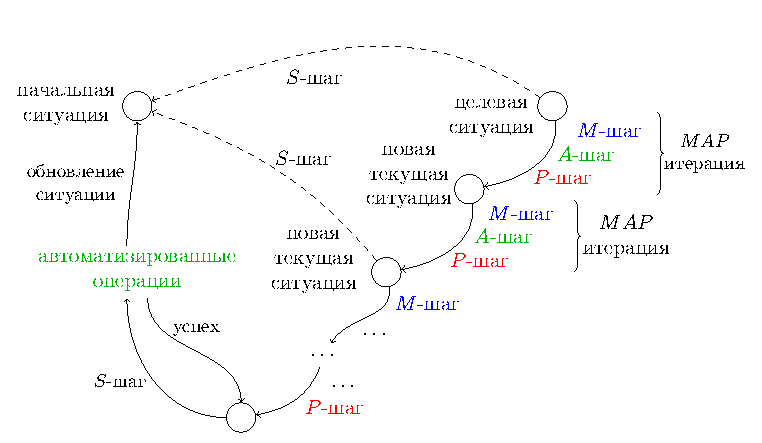
\includegraphics[width=\textwidth]{algo/ru/beh_plan2_ru}
		\caption{Схема процесса планирования поведения}	
		\label{fig:plan_algo}	
	\end{figure}
	
	Кратко, MAP-алгоритм осуществляет итеративную генерацию новых каузальных матриц $z_{next}$ личностных смыслов на основе текущей активной матрицы $z_{cur}$ до тех пор, пока не будет достигнуто предельное количество шагов $i_{max}$ (шаг \ref{alst:exit}) или не будет целиком активирован начальная матрица $z_{start}$ (шаг \ref{alst:suc_exit}), соответствующей личностному смыслу $a_{start}$ начальной ситуации. В качестве текущей активной каузальной матрицы для первой итерации выступает матрица, соответствующая личностному смыслу целевой ситуации $z_{goal}^a$ (шаг \ref{alst:start_iter}). После завершения выполнения всех итераций, найденные планы сортируются по длине (шаг \ref{alst:sort}) и самый короткий из них является решением задачи планирования в знаковой картине мира (шаг \ref{alst:return}).
	
	Первым этапом в MAP-итерации является S-этап. Его суть заключается в том, что в картине мира интеллектуального агента производится поиск прецедентов, т.е. поиск действий, которые совершались в текущих условиях $z_{cur}$. Для этого просматриваются все знаки в картине мира $S$ и их личностные смыслы $a(s)$ (шаги \ref{alst:check_wm}--\ref{alst:check_a}). Если текущие условия $z_{cur}$ удовлетворяются матрицей $z_a$, то список прецедентов $\hat A_{case}$ пополняется результатом распространения активности по сети личностных смыслов от знака $s$ на расстояние $d_a$ (шаг \ref{alst:search_case}).
	
	\begin{algorithm}
		\begin{algorithmic}[1]
			\algrestore{algst:store1}
			\Function{map\_iteration}{$z_{cur}$,$z_{start}$, $Plan_{cur}$, $i$}
	\If{$i \geq i_{max}$}\label{alst:exit}
		\State\Return $\varnothing$
	\EndIf
	
	\State $\hat A_{case}:=\varnothing$ \Comment{Список прецедентов}
	
	\Statex\Comment{$S$-этап}
	\Statex\Comment{Поиск прецедентов выполнения действий в текущих условиях}
		
	\ForAll{$s\in S$} \label{alst:check_wm}
		\ForAll{$z_a\in a(s)$}\label{alst:check_a}
			\If{$z_a \geq z_{cur}$}
				\State $\hat A_{case} = \hat A_{case} \cup \varphi_a^\uparrow(s,d_a)$ \label{alst:search_case}
			\EndIf
		\EndFor
	\EndFor
			\algstore{algst:store2}
		\end{algorithmic}
	\end{algorithm}
	
	Далее в MAP-алгоритме следует M-этап, на котором происходит распространение активности по сети личностных смыслов на расстояние $d_a$ с целью активации всех знаков, связанных с текущей ситуацией (шаг \ref{alst:state_def}). Элементы полученного множества каузальных матриц $A^*$ служат отправными точками для распространения активности по сети значений: для каждой матрицы $z_a$ с помощью функции связывания $\Psi_a^m$ определяется необходимый узел на каузальной сети значений, от которого активность распространяется на расстояние $d_m$ (шаг \ref{alst:search_act}). Если активированные матрицы являются каузальными, то они добавляются в множество активных значений $M^*$ (шаг \ref{alst:add_signif}).
	
	\begin{algorithm}
		\begin{algorithmic}[1]
			\algrestore{algst:store2}
			\Statex\Comment{$M$-этап}
\Statex\Comment{Распространение активности вниз по сети личностных смыслов}
\State $A^* = \varphi_a^\downarrow(z_{cur}, d_a)$\label{alst:state_def}
\State $M^*=\varnothing$
\ForAll{$z_a\in A^*$}
	\Statex\Comment{Распространение активности вверх по сети значений}
	\ForAll{$z_m\in \varphi_m^\uparrow(s(z_a), d_m)$} \label{alst:search_act}
		\If{$I^e(z_m) \not= \varnothing$}
			\State $M^* := M^*\cup\{z_m\}$ \label{alst:add_signif}
		\EndIf
	\EndFor
\EndFor

			\algstore{algst:store3}
		\end{algorithmic}
	\end{algorithm}
	
	Затем переходим к A-этапу, на котором происходит генерация каузальных матриц на сети личностных смыслов, которые представляют специфицированные относительно текущих условий $z_{cur}$ действия, определяемые активными значениями из множества $M^*$. Для этой цели служат шаги \ref{alst:a_spread_m}--\ref{alst:a_gen_a}, в которых распространение активности на каузальной сети значений на расстояние $d_m$ приводит к активации множества значений $M^*$ знаков, связанных с ролевой структурой процедурной матрицы $z_m$, а затем с помощью функции связывания $\Psi_m^a$ происходит генерация новой каузальной матрицы на сети личностных смыслов, которая копирует значение $z_m^*$ с замещением абстрактных знаков-ролей объектными знаками, связанными с ролями отношением класс-подкласс. Затем на A-шаге происходит отбор тех каузальных матриц, которые представляют действия, выполнимые в текущих условиях $z_{cur}$ (шаги \ref{alst:a_shift}--\ref{alst:a_filter}). Для этого удаляются все каузальные матрицы, эффекты которых не включены в текущую ситуацию (напомним, что планирование осуществляется в обратном направлении). В заключение A-этапа выполняется одна из операций в картине мира $\theta_a$, осуществляющая в данном случае метарегулирование - проверку некоторой эвристики, которая может выражать, например, то правило, что нельзя повторять одинаковые действия, или лучше выполнить то действие, которое быстрее всего приближает к начальным условиям $z_{start}$ (шаг \ref{alst:a_meta}). Любое эвристическое правило также представимо в виде каузальной матрицы личностного смысла знака, представляющего внутреннюю стратегию планирования своего поведения.
		
	\begin{algorithm}
		\begin{algorithmic}[1]
			\algrestore{algst:store3}
			\Statex\Comment{$A$-этап}
\State $\hat A_{gen}=\varnothing$
\ForAll{$z_m\in M^*$}
	\Statex\Comment{Распространение активности вниз по сети значений}
	\State $\hat M^*=\varphi_m^\downarrow(z_m, d_m)$\label{alst:a_spread_m}
	\ForAll{$z_m^*\in \hat M^*$}
		\State $\hat A_{gen} := \hat A_{gen}\cup\{\Psi_m^a(z_m^*)\}$ \label{alst:a_gen_a}
	\EndFor
\EndFor
\Statex\Comment{Совмещение активности образованных смыслов и текущей ситуации}
\State $\hat A = \hat A_{gen}\cup \hat A_{case}$
\ForAll{$z_a\in \hat A$}
	\State $z_{shift}=(e_i|i\in I^e(z_a))$ \label{alst:a_shift}
	\If{$z_{cur} \not\geq z_{shift}$}
		\State $\hat A = \hat A\setminus\{z_a\}$ \label{alst:a_filter}
	\EndIf
\EndFor
\Statex\Comment{Метакогнитивная проверка эвристики}
\State $\hat A=\{\theta_a(z_a)|z_a\in\hat A\}$ \label{alst:a_meta}
\If{$\hat A = \varnothing$}
	\State\Return $\varnothing$
\EndIf

			\algstore{algst:store4}
		\end{algorithmic}
	\end{algorithm}
	
	Завершается MAP-алгоритм P-этапом. Здесь для каждой сгенерированной каузальной матрицы $z_a$, представляющей некоторое действие, формируется новая ситуация $Sit_{next}$, которая является результатом обратного применения действия в текущих условиях $z_{cur}$. Обратное применение (шаг \ref{alst:p_next_gen}) заключается в формировании каузальной матрицы $z_{next}$, состоящей из событий, являющихся либо колонками-условиями действия $e_i\in\{e_k|e_k\in z_a, k\in I^c(z_a)$, либо принадлежащих текущей активной каузальной матрице и не являющихся колонками-эффектами действия $e_i\in z_{cur} \land e_i\not\in\{e_j|e_j\in z_a, j\in I^e(z_a)\}$. Именно этот этап представляет собой включение подпроцесса целеполагания в процесс планирования. Новая ситуация становится новой целью в следующей итерации. В текущий план $Plan_{cur}$ добавляется пара текущие условия - применимое действие $\langle z_{cur}, z_a\rangle$. Если новая ситуация не покрывает стартовую ситуацию (шаг \ref{alst:suc_exit}), то итерации продолжаются с новой текущей ситуацией, пополняя все множество генерируемых планов $Plans_{fin}$.
	
	Константы $d_a, d_m$, которые определяют глубину распространения активности в каузальных сетях, являются параметрами алгоритма и задают внутреннюю характеристику носителя картины мира, различаясь от агента к агенту. Обычно в модельных экспериментах эти параметры не превышают 5. 
		
	\begin{algorithm}
		\begin{algorithmic}[1]
			\algrestore{algst:store4}
				\Statex\Comment{$P$-этап}
	\State $Plans_{fin} := \varnothing$
	\ForAll{$z_a\in\hat A$}
		\State $Plan_{cur} = Plan_{cur}\cup\{\langle z_{cur}, z_a\rangle\}$
		\Statex\Comment{Генерация новой ситуации - применение действия} 		
		\State $z_{next} := (e_i|(e_i\in z_{cur} \land e_i\not\in\{e_j|e_j\in z_a, j\in I^e(z_a)\}) \lor e_i\in\{e_k|e_k\in z_a, k\in I^c(z_a)\})$\label{alst:p_next_gen}
		\State $Sit_{next} = \langle id_{next}, \varnothing, \varnothing, \{z_{next}\} \rangle$
		\If{$z_{next} \geq z_{start}$}\label{alst:suc_exit}
			\State $Plans_{fin} = Plans_{fin}\cup\{Plan_{cur}\}$
		\Else
			\State $Plans_{rec}$ := \Call{map\_iteration}{$z_{next}$,$z_{start}$, $Plan_{cur}$, $i+1$}
			\State $Plans_{fin} = Plans_{fin}\cup Plans_{rec}$
		\EndIf
	\EndFor
	
	\State\Return $Plans_{fin}$
\EndFunction
		\end{algorithmic}
	\end{algorithm}
	
	\subsection{Модельный пример: мир кубиков}\label{sec:example}
	
	Продемонстрируем работу представленного алгоритма планирования поведения с помощью модельного эксперимента, доменом планирования для которого выступает широко известный в области автоматического планирования пример <<мир кубиков>> \cite{Gupta1992}. Описание домена на языке PDDL \cite{Gerevini2009} состоит из определения типа (\textit{blocks}), четырех предикатов (\textit{ontable}, \textit{clear}, \textit{handempty}, \textit{holding}) и четырех действий (\textit{pick-up}, \textit{put-down}, \textit{stack}, \textit{unstack}) (см. табл. \ref{tab:domain}).
	
	\begin{table}
		\footnotesize
		\centering
		\begin{tabular}{|p{0.3\textwidth}|p{0.3\textwidth}|p{0.3\textwidth}|}
			\hline
			(define (\textbf{domain BLOCKS})
			
			(:requirements :strips :typing)
			
			(:types block)
			
			(:predicates (on ?x - block ?y - block)
			
			(ontable ?x - block)
			
			(clear ?x - block)
			
			(handempty)
			
			(holding ?x - block)
			)
			&
			(:\textbf{action pick-up}
			
			:parameters (?x - block)
			
			:precondition (and (clear ?x) (ontable ?x) (handempty))
			
			:effect
			
			(and (not (ontable ?x))
			
			(not (clear ?x))
			
			(not (handempty))
			
			(holding ?x)))
			&
			(:\textbf{action put-down}
			
			:parameters (?x - block)
			
			:precondition (holding ?x)
			
			:effect
			
			(and (not (holding ?x))
			
			(clear ?x)
			
			(handempty)
			
			(ontable ?x)))
			\\
			\hline
			(:\textbf{action stack}
			
			:parameters (?x - block ?y - block)
			
			:precondition (and (holding ?x) (clear ?y))
			
			:effect
			
			(and (not (holding ?x))
			
			(not (clear ?y))
			
			(clear ?x)
			
			(handempty)
			
			(on ?x ?y)))
			&
			(:\textbf{action unstack}
			
			:parameters (?x - block ?y - block)
			
			:precondition (and (on ?x ?y) (clear ?x) (handempty))
			
			:effect
			
			(and (holding ?x)
			
			(clear ?y)
			
			(not (clear ?x))
			
			(not (handempty))
			
			(not (on ?x ?y)))))
			&
			(define (\textbf{problem BLOCKS-4-0})
			
			(:domain BLOCKS)
			
			(:objects D B A C - block)
			
			(:INIT (CLEAR C) (CLEAR A) (CLEAR B) (CLEAR D) (ONTABLE C) (ONTABLE A)
			
			(ONTABLE B) (ONTABLE D) (HANDEMPTY))
			
			(:goal (AND (ON D C) (ON C B) (ON B A)))
			)\\
			\hline
		\end{tabular}
		\caption{Описание домена планирование <<мир кубиков>> и задачи построения башни.}
		\label{tab:domain}
	\end{table}
	
	Приведем пример решения с использованием MAP-алгоритма следующей задачи планирования - построение башни из четырех кубиков, лежащих на столе (табл. \ref{tab:domain}). Фрагмент каузальной сети на личностных смыслах, задающего каузальную матрицу смысла начальной ситуации с именем \textit{start}, приведен на рис. \ref{fig:start_sit}. У каждого отдельного кубика (\textit{a}, \textit{b}, \textit{c}, \textit{d}) одна каузальная матрица в узле сети, в то время как для предикатов \textit{clear} и \textit{ontable} имеется по четыре матрице в узле, т.к. они принимают участие в событиях с разными кубиками. Например, матрицы знака \textit{clear} присутствуют в 1, 3, 5 и 7 столбцах матрицы знака \textit{start} одновременно с кубиками \textit{a}, \textit{b}, \textit{c}, \textit{d} соответственно, что означает, что на всех кубиках не лежат другие кубики.
	
	\begin{figure}
		\centering
		\includegraphics[width=0.75\textwidth,page=3]{examples/plan/plan_nets}
		\includegraphics[width=0.6\textwidth,page=2]{examples/plan/block_world}
		\caption{Начальная ситуация: все четыре кубика лежат на столе.}	
		\label{fig:start_sit}	
	\end{figure}
	
	На рис. \ref{fig:goal_sit} представлена целевая ситуация, в которой все четыре кубика составлены в башню: кубик \textit{d} находится на столе, кубик \textit{c} - на \textit{d}, \textit{b} - на \textit{c}, и, наконец, на самом верху - кубик \textit{a}. Предикат \textit{on}, который задает отношение <<находится на>> может быть представлен в виде процедурный каузальной матрицы, чтобы явно продемонстрировать несимметричность этого отношения, хотя использование объектной матрицы никак не влияет на результат. Здесь также от каждого кубика в ситуации участвует одна каузальная матрица, а предикат \textit{on} представлен в виде узла с тремя каузальными матрицами, т.к. участвует в матрице знака целевой ситуации \textit{goal} в различных столбцах с тремя различными кубиками.
	
	\begin{figure}
		\centering
		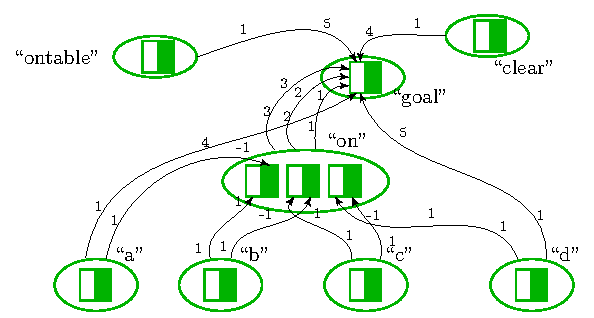
\includegraphics[width=0.73\textwidth,page=1]{examples/plan/plan_nets}
		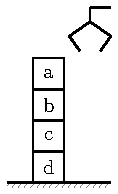
\includegraphics[width=0.23\textwidth,page=1]{examples/plan/block_world}
		\caption{Целевая ситуация: башня из четырех кубиков.}	
		\label{fig:goal_sit}	
	\end{figure}
	
	На рис. \ref{fig:stack_sig} представлен фрагмент каузальной сети на значениях, представляющий собой элементы процедурной каузальной матрицы знака \textit{stack} и отношения <<класс-подкласс>> объектов-кубиков, класса \textit{block} и ролей в действии \textit{stack}: \textit{block?x} (аналог семантической роли <<объект>>) \textit{block?y} (аналог семантической роли <<директив>>). Здесь необходимо отметить, что метка $\epsilon_1$ ребра $v$ (индекс исходной матрицы узла, из которого исходит ребро $v$) в случае отношения <<класс-подкласс>> (\textit{a}$\rightarrow$\textit{block}, \textit{block}$\rightarrow$\textit{block?x}) принимает специальное нулевое значение, что означает, что исходной может быть любая казуальная матрица данного узла. Иными словами, роль \textit{block?x} может играть любой из кубиков \textit{a}, \textit{b}, \textit{c} или \textit{d}.
	
	\begin{figure}
		\centering
		\includegraphics[width=0.7\textwidth,page=2]{examples/plan/plan_nets}
		\includegraphics[width=0.27\textwidth,page=3]{examples/plan/block_world}
		\caption{Фрагмент каузальной сети на значениях: представление действия \textit{stack}.}	
		\label{fig:stack_sig}	
	\end{figure}
	
	Рассмотрим этапы MAP-алгоритма: S, M, A и P-этапы - на первой итерации алгоритма. Рассмотрим простейший случай, когда наш интеллектуальный агент не накопил опыта действования в условиях данной задачи. В следствие этого на S-этапе множество прецедентов $\hat A_{case}$ будет пусто. С учетом того, что планирование осуществляется в обратном направлении, на первом M-этапе мы рассматриваем целевую ситуацию как текущую активную матрицу предсказания $z_{cur}$ и распространение от нее активности вниз по сети личностных смыслов будет активировать множество $A^*$, совпадающее с фрагментом, изображенным на рис.\ref{fig:start_sit}. В множество значений $M^*$ попадут значения знаков, представляющих кубики \textit{a},\textit{b},\textit{c},\textit{d} - это все связанные с ними по сети значений процедурные знаки \textit{stack}, \textit{unstack}, \textit{pick-up}, \textit{put-down}. На рис. \ref{fig:unstack_gen} слева представлен фрагмент каузальный сети на значениях, включающий процедурную матрицу знака \textit{unstack}. Для активации матрицы знака \textit{unstack} от матрицы знака \textit{a} достаточно использовать в качестве константы $d_m$ значение в три ребра.
	
	\begin{figure}
		\centering
		\includegraphics[width=0.48\textwidth,page=5]{examples/plan/plan_nets}
		\includegraphics[width=0.48\textwidth,page=4]{examples/plan/plan_nets}
		\caption{Распространение активности по сети значений, генерация личностного смысла знака \textit{unstack}.}	
		\label{fig:unstack_gen}	
	\end{figure}
	
	На A-этапе происходит генерация новых каузальных матриц $\hat A_{gen}$ в сети личностных смыслов путем распространения активности вниз по сети значений. Пример такого распространения, в результате которого образуется новая каузальная матрица знака \textit{unstack}, представлен на рис. \ref{fig:unstack_gen} справа. Новая каузальная матрица на сети личностных смыслов является копией соответствующей матрица на сети значений с заменой ссылок, указывающих на знаки-роли, на ссылки, указывающие на объектные не абстрактные знаки, представляющие кубики. В нашем примере будет сгенерирована матрица, соответствующая действию \textit{unstack}(\textit{a}, \textit{b}) - снять кубик \textit{a} с кубика \textit{b}. На данном этапе будет сформировано по четыре матрицы для одноместных действий и двенадцать - для двухместных.
	
	В завершение A-этапа эффекты построенных процедурных матриц проверяются на применимость в условиях текущей ситуации и среди применимых действий отбираются те, которые удовлетворяют некоторому метакогнитивному правилу (эвристике) $\theta_a$. В нашем примере, единственным применимым действием из всех сформированных вариантов будет действие \textit{unstack}(\textit{a},\textit{b}). В качестве эвристики может быть использовано жадное правило: выбираем те действия, которые максимально быстро приближают к успеху (новая ситуация имеет больше общих признаков с целевой).
	
	В конце итерации, на P-этапе, генерируется новая каузальная матрица $z_{next}$ в сети личностных смыслов знака, представляющего следующую ситуацию планирования. В нашем примере новая текущая ситуация будет совпадать с предыдущей за исключение того, что кубик \textit{a} теперь находится в манипуляторе, а на кубике \textit{b} теперь ничего не находится. В текущий план $Plan_{cur}$ добавляется пара $\langle z_{cur}, z_a \rangle$ каузальных матриц текущей ситуации и выбранного действия. Т.к. новая ситуация не включает в себя стартовую ситуации начинаем новую итерацию.
	
	В результате работы MAP-алгоритма в нашем примере будет получен план из 6 действий: \textit{pick-up}(\textit{c}), \textit{stack}(\textit{c},\textit{d}), \textit{pick-up}(\textit{b}), \textit{stack}(\textit{b},\textit{c}), \textit{pick-up}(\textit{a}), \textit{stack}(\textit{a},\textit{b}). В завершение работы агента над этой задачей он сохраняет прецедент планирования в своей картине мира: он сохраняет начальную и конечную ситуацию в виде новых знаков и образует новый процедурный знак, который можно назвать как <<построить башню>>. Единственным признаком в столбце условий данного знака будет начальная ситуация, единственным признаком в столбце эффектов - целевая ситуация. После этого интеллектуальный агент сможет решить ту же задачу, найдя на S-этапе необходимое действие, которое сразу приведет к цели. Такая же ситуация может возникнуть и в другой задаче по ходу ее решения, что приведет к сокращению пространства поиска подходящих действий.
		
	\subsection{Выводы}
	
	В классической символьной постановке задачи планирования в искусственном интеллекте возникает проблема совмещения символьных алгоритмов планирования с методами обучения, сохраняющими как опыт планирования, так и обеспечивающими адаптацию действий к новым условиям. Данная проблема смыкается с проблемой символизации - привязки используемых в классическом способе представления знаний символов к реальным объектам, процессам и свойствам внешней среды. Особенно остро данные проблемы проявляется при реализации обучаемых робототехнических систем, для которых важно сопоставлять символы, используемые при концептуальном планировании с данными, поступающими от сенсоров. При этом, когда перед сложной технической системой ставится задача планирования в довольно широком спектре условий, в том числе и коалиционных, подходы с заранее сформированной, хоть и пополняемой, базой знаний показывают свою неэффективность. Способ представления знаний, на котором базируются функции управления интеллектуальным агентом, должен изначально поддерживать возможность привязки символов к данным сенсоров и поддерживать как представление внутренней информации, так и обобщенной, согласованной с другими участниками коалиции информации. 
	
	В настоящем проекте эти задачи решаются с использованием знаковой картины мира. Исследована структура внутренней процедурной компоненты элементов семиотического представления знаний (знаков) интеллектуального агента. Исследована взаимосвязь процессов целеполагания и процесса функционирования внутренней процедурной компоненты знака. Представлен оригинальный метод планирования (MAP-алгоритм), который использует и сохраняет прецедентную информацию в процессе синтезе плана. MAP-алгоритм включает в себя этап целеполагания - генерации новой цели на основе предыдущего опыта и текущей ситуации. Используемый четырехкомпонетный элемент картины мира (знак) позволяет кодировать не только информацию о внешней среде, но и внутренние характеристики и мотивационно-потребностные свойства, а так же общие коллективные знания. Представленный алгоритм также может быть использован и для составления коалиционных планов. Для демонстрации работы MAP-планирощика приведен модельный пример составления плана для одной из задач <<мира кубиков>>. Программная реализация и модельные эксперименты представлены в репозитории \href{https://github.com/cog-isa/map-planner}{https://github.com/cog-isa/map-planner}.
	
	\printbibliography[heading=none,resetnumbers=true]
	
	\section{Вклад каждого члена коллектива в выполнение Проекта в 2016 году}
	Проект выполнялся индивидуально без привлечения сторонних лиц для выполнения основных работ.
	
	\section{Участие в 2016 году в научных мероприятиях по тематике Проекта}
	\begin{enumerate}
		\item 22.04.2016 --- устный доклад <<Biologically and psychologically inspired modelling in BICA>>, First International Early Research Career Enhancement School on Biologically Inspired Cognitive Architectures <<Fierces on BICA>> (21-24 апреля 2016, Москва).
		\item 23.06.2016 --- устный доклад <<Моделирование процесса планирования поведения в знаковой картине мира>>, Седьмая международная конференция по когнитивной науке (20-24 июня 2016, Светлогорск).
	\end{enumerate}
	\section{Библиографический список всех публикаций по Проекту, опубликованных в 2016 году, в порядке значимости: монографии, статьи в научных изданиях, тезисы докладов и материалы съездов, конференций и т.д.}
	\nocite{*}
	\printbibliography[heading=none,keyword={myart},resetnumbers=true]
	\printbibliography[heading=none,keyword={myconf}]
	\printbibliography[heading=none,keyword={myth}]
\end{document}